\documentclass[varwidth=true, border=2pt]{standalone}

\usepackage{tikz}
\usetikzlibrary{decorations.fractals}
\usepackage{pgfplots}

\begin{document}
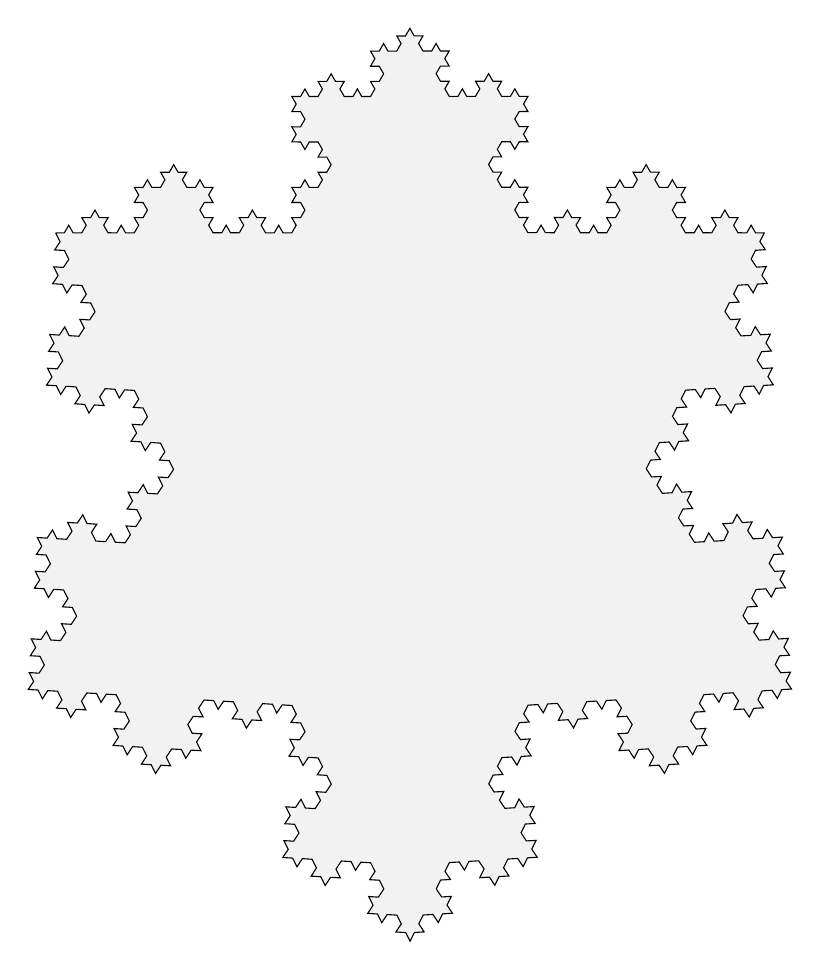
\begin{tikzpicture}[scale=3,decoration=Koch snowflake]
% \draw[fill=gray!10] { { { { (0,0) -- (3,0) -- (1.5,-3) -- (0,0)}}}};
% \draw[fill=gray!10] { { { decorate{ (0,0) -- (3,0) -- (1.5,-3) -- (0,0)}}}};
% \draw[fill=gray!10] { { decorate{ decorate{ (0,0) -- (3,0) -- (1.5,-3) -- (0,0)}}}};
% \draw[fill=gray!10] { decorate{ decorate{ decorate{ (0,0) -- (3,0) -- (1.5,-3) -- (0,0)}}}};
\draw[fill=gray!10] decorate{ decorate{ decorate{ decorate{ (0,0) -- (3,0) -- (1.5,-3) -- (0,0)}}}};
\end{tikzpicture}
\end{document}
